\documentclass[11pt]{article}

\usepackage{graphicx}

\oddsidemargin=.25in
\evensidemargin=.25in
\textwidth=6in
\topmargin=0in

\parindent=0in

\begin{document}

\centerline {\Large \bf Kobby Editor: Collaborative Editing Instructions}
\centerline {Written by Gregory Haynes}

\paragraph{}The central feature of Kobby is the ability to host and join collaboratively edited documents.  Collaborative editing allows multiple people to work on the same document simultaneosly, similar to how several people could write on a large sheet of paper simultaneusly.

\begin{figure}[tbh]
\begin{center}
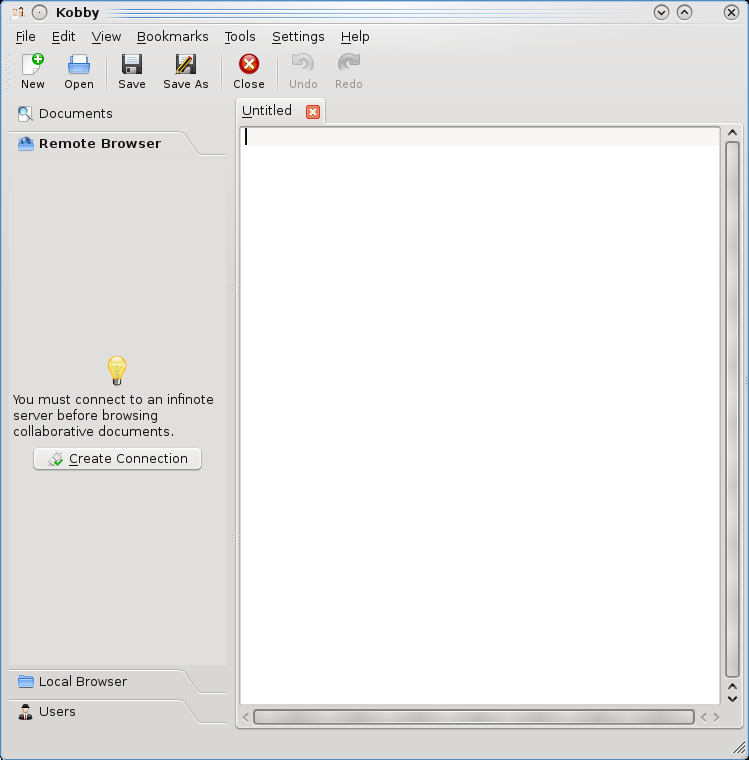
\includegraphics[width=.7\textwidth]{kobbymain.png}
\end{center}
\caption{Kobby Editor Main Window}
\end{figure}

\paragraph{}Collaborative editing in Kobby is done by having each document ``hosted'' on one persons comuter, while all the other users connect to that computer and edit the same document.  Thinking in terms of the drawing on paper example, in order for everyone to draw on the same paper everyone must agree on which sheet of paper will be used.  Once a document has been created on the host computer, users can then join the document to begin editing.  This instruction will walk through the process of creating a document on a host computer, and then joining that document to begin collaborative editing.

\paragraph{Before you begin} you must have a recent version of Kobby installed on your computer.  If you do not know how to install Kobby, instructions for doing this can be found on the Kobby website at http://greghaynes.github.com/kobby.

\paragraph{}

\end{document}